\documentclass[11pt]{article}

% Packages
\usepackage[utf8]{inputenc}
\usepackage[margin=1in]{geometry}
\usepackage{amsmath}
\usepackage{amssymb}
\usepackage{physics}
\usepackage{graphicx}
\usepackage[authoryear]{natbib}
\setcitestyle{authoryear,round,aysep={}}
\let\cite\citep
\usepackage{hyperref}
\usepackage{fancyhdr}

% Header and Footer
\pagestyle{fancy}
\fancyhf{}
\rhead{\thepage}
\lhead{Astronomical Research Proposal}

% Title
\title{ \Large Research Proposal: \\
 Validation of 7DT Photometric Redshift Performance in the COSMOS Field and Its Applicability to Weak Lensing}
\author{Han Kyul Seo}
\date{\today}

\begin{document}

\maketitle

\section{Introduction}

In recent astronomy, statistical studies of galaxy evolution and the large-scale structure of the Universe based on wide-field observations have become increasingly important \cite{weinberg2013observational}. In particular, the development of large imaging surveys containing vast numbers of extragalactic sources has enabled not only detailed studies of individual objects but also cosmological analyses based on the spatial distribution of large galaxy samples. In such studies, one of the key observables is the redshift of galaxies. Redshift information is essential for estimating the line-of-sight distribution of galaxies, and it allows us to investigate the three-dimensional distribution of galaxies and the growth of cosmic structure \cite{hamilton1998linear}.

In this context, weak lensing has emerged as an important tool in modern observational cosmology \cite{Mandelbaum2018}. By statistically analyzing the subtle shape distortions of background galaxies induced by foreground matter distribution, weak lensing provides constraints on the large-scale matter distribution and cosmological parameters. However, the reliability of weak lensing analyses depends strongly on the redshift information of the background galaxy sample. In other words, not only accurate shape measurements but also sufficiently reliable estimates of the redshift distribution of source galaxies are required in order to derive meaningful cosmological conclusions \cite{Salvato2019,Huterer2013}.

The most traditional and direct method for measuring galaxy redshifts is spectroscopy. Spectroscopic observations determine redshifts with high precision by directly measuring the wavelength shifts of emission lines, absorption features, and spectral breaks \cite{Salvato2019}. However, spectroscopy requires substantial observing time and cost, and it is difficult to apply to the entirety of a wide-field survey containing a large number of faint extragalactic sources. For this reason, photometric redshift methods, or photo-z, which can be applied to much larger samples at lower observational cost, have become widely used in modern large-scale imaging surveys \cite{Salvato2019}.

Photo-z estimates redshift using photometric measurements obtained over multiple wavelength bands, which provide a coarse sampling of the spectral energy distribution of a galaxy \cite{Salvato2019}. This approach has the advantage of being applicable to far larger samples than spectroscopy and has effectively become indispensable in modern large imaging surveys. However, because photo-z relies intrinsically on lower spectral resolution than spectroscopy, it can produce redshift scatter, systematic bias, and catastrophic outliers \cite{Salvato2019,Dahlen2013}. These errors can become an important source of systematic uncertainty in studies that are sensitive to redshift calibration, such as weak lensing, and therefore the accuracy and applicability of photo-z must be carefully validated \cite{Huterer2013,LSSTDESC2018}.

One approach proposed to mitigate these limitations is the use of medium-band or narrow-band observing strategies, which provide denser wavelength sampling than broad-band photometry \cite{Wolf2003,Cardamone2010,Benitez2014}. Because such systems can trace major spectral features in galaxy SEDs, such as the 4000~\AA\ break and strong emission lines, more effectively than broad-band filters alone, they can potentially yield more accurate photo-z estimates. Indeed, previous studies such as COMBO-17, MUSYC, and J-PAS have demonstrated that medium-band or narrow-band observations can significantly improve photo-z performance \cite{Wolf2003,Cardamone2010,HernanCaballero2021}.

The 7-Dimensional Telescope (7DT) is a system designed to actively exploit this medium-band observational strategy \cite{Ko2025}. By employing densely spaced medium-band filters, 7DT is designed to trace galaxy SEDs more finely than conventional broad-band surveys. In particular, recent forecast studies have suggested that the medium-band system of 7DT and 7DS may provide superior photo-z performance compared to broad-band photometry \cite{Ko2025}. However, such results have been based primarily on mock catalogs, and it remains to be verified whether comparable performance can be achieved with real observational data.

Therefore, the purpose of this study is to test the performance of medium-band-based photo-z using actual 7DT observations. In particular, using data from the COSMOS field, I aim to evaluate how well SEDs constructed from 7DT photometry can reproduce redshift estimates when compared with spectroscopic redshifts or other external reference data. Through this analysis, I seek to investigate the potential of the 7DT medium-band system for future photo-z catalog construction and for applications to extragalactic studies such as weak lensing, while also discussing the limitations and possible directions for improvement in practical use.


\section{Previous research}
A previous study forecasted the photometric redshift performance of the 7DT medium-band filter system \cite{Ko2025}. In that work, the authors constructed a mock catalog rather than using a real observed catalog, and evaluated the photo-z performance at different survey depths using EAZY. They showed that the 7DT medium-band data can improve photo-z accuracy by effectively capturing the 4000~\AA\ break and emission-line features.

The purpose of this study is to extend that previous work to real observational data. In other words, while the previous study predicted the potential of 7DT using simulated data, this study directly tests the photo-z performance of 7DT using actual observations and examines whether the advantages of the medium-band system can be reproduced in practice.


\section{Objectives}

This study has three main objectives:
\begin{enumerate}
    \item Construct a real multi-band photometric catalog based on 7DT observations of the COSMOS field.
    \item Validate the photometric redshift performance of 7DT by comparing photo-z estimates with external reference data.
    \item Assess whether the resulting catalog is suitable for future weak lensing applications.
\end{enumerate}

\section{Data}

This study uses calibrated observational data provided by 7DT. The data set consists of multi-band imaging data for the COSMOS 1-4 fields and the corresponding filter response functions, and the images are provided in FITS format. Since the data are already calibrated, this study focuses on subsequent photometric analysis and catalog construction rather than on raw data reduction.

Each field was observed with the 7DT medium-band filter system, enabling multi-wavelength photometric measurements of the same sources. The provided filter response functions will be used in the later stages of flux conversion, SED construction, and SED fitting. Using these real observational data, this study aims to construct a multi-band photometric catalog and to assess the spectral sampling capability and photometric redshift applicability of 7DT.

Table~\ref{tab:cosmos_fields} summarizes the approximate sky coverage of the four COSMOS fields used in this study.
The 7DT filter set used in this study consists of the medium-band filters
\(m400\), \(m425\), \(m450\), \(m475\), \(m500\), \(m525\), \(m550\), \(m575\),
\(m600\), \(m625\), \(m650\), \(m675\), \(m700\), \(m725\), \(m750\),
\(m775\), \(m800\), \(m825\), \(m850\), and \(m875\).
The number in each filter name indicates the central wavelength of the filter in nanometers.
The corresponding transmission curves will be presented in Figure~\ref{fig:filter_curves}.

\begin{table}[htbp]
\centering
\caption{Approximate sky coverage of the COSMOS 1--4 fields}
\label{tab:cosmos_fields}
\begin{tabular}{llll}
\hline
Field & RA range & Dec range \\
\hline
COSMOS 1 & 09:56:20.18 -- 10:02:03.82 & +01:28:22.88 -- +02:25:36.03 \\
COSMOS 2 & 09:56:20.10 -- 10:02:03.90 & +02:01:22.72 -- +02:58:35.87 \\
COSMOS 3 & 09:58:44.18 -- 10:04:27.82 & +01:28:22.88 -- +02:25:36.03 \\
COSMOS 4 & 09:58:44.10 -- 10:04:27.90 & +02:01:22.72 -- +02:58:35.87 \\
\hline
\end{tabular}
\end{table}

\begin{figure}[htbp]
\centering
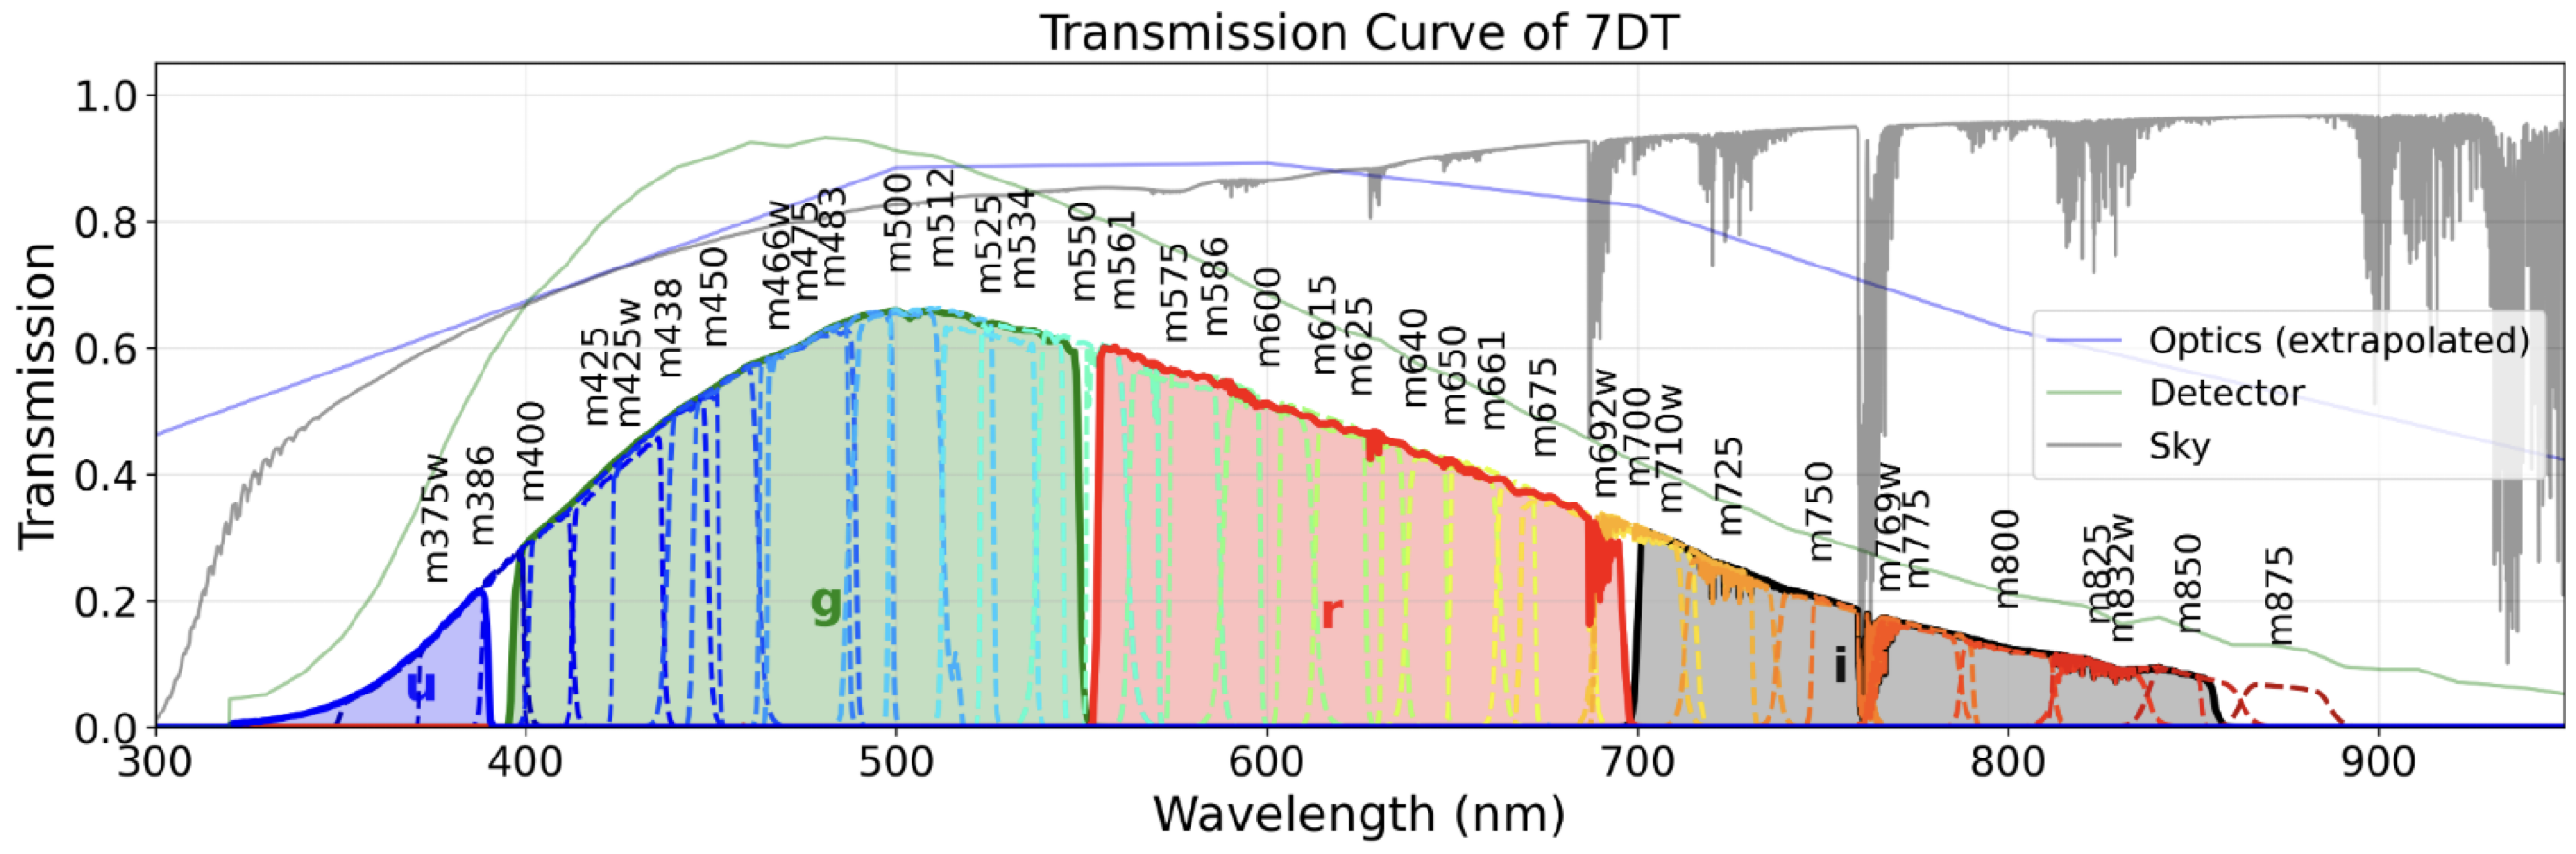
\includegraphics[width=0.8\textwidth]{filter_curves.png}
\caption{Transmission curves of the 7DT medium-band filters used in this study. The curves were provided by the 7DT team.}
\label{fig:filter_curves}
\end{figure}


\section{Methodology}

First, photometry will be performed on each 7DT band image using Source Extractor++. The catalogs produced from individual bands will then be matched across bands to construct a master multi-band catalog. In this step, only sources with sufficiently reliable detections will be retained, and the measured magnitudes will be converted into fluxes for subsequent analysis.

After constructing the catalog, data quality checks will be carried out. In particular, sources showing anomalous flux values in specific bands or SED shapes inconsistent with adjacent wavelength bands will be inspected as suspicious sources. In addition, whenever possible, the 20-band SEDs obtained from 7DT will be compared with SED information from existing surveys in order to assess how well the 7DT photometry reproduces meaningful spectral features.

Next, SED fitting will be performed using \textsc{CIGALE}, with the 7DT filter response functions incorporated into the fitting process. This step is intended to test whether physically plausible SEDs can be reconstructed from the 7DT photometric data alone. For sources with external SED information or reference photometric data, the fitted results will be compared with those data in order to evaluate the reliability of the reconstructed SEDs.

Finally, photometric redshifts will be derived from the 7DT-based photometric catalog, and their performance will be quantitatively evaluated. For this purpose, the estimated photometric redshifts $z_{\mathrm{phot}}$ will be compared with reference redshifts $z_{\mathrm{ref}}$, taken from spectroscopic measurements or other sufficiently reliable external redshift data when available. Following \citet{Ko2025}, the photo-\textit{z} performance will be characterized using three complementary metrics: the catastrophic failure fraction $\eta$, the normalized median absolute deviation $\sigma_{\mathrm{NMAD}}$, and the bias $b$.

The redshift residual is defined as
\[
\Delta z = z_{\mathrm{ref}} - z_{\mathrm{phot}} .
\]
Using this quantity, the catastrophic failure fraction is defined as
\[
\eta = \mathrm{fraction}\left( \frac{|z_{\mathrm{ref}} - z_{\mathrm{phot}}|}{1+z_{\mathrm{ref}}} > 0.15 \right) ,
\]
which measures the fraction of sources whose photometric redshifts are severely misestimated. The overall scatter of the photo-\textit{z} estimates will be quantified by
\[
\sigma_{\mathrm{NMAD}}
=
1.48 \times
\mathrm{median}
\left(
\frac{|\Delta z - \mathrm{median}(\Delta z)|}{1+z_{\mathrm{ref}}}
\right) ,
\]
while the systematic offset will be evaluated through the bias,
\[
b
=
\left\langle
\frac{z_{\mathrm{phot}} - z_{\mathrm{ref}}}{1+z_{\mathrm{ref}}}
\right\rangle .
\]

These metrics will be examined for the full sample and, when possible, as a function of magnitude and source quality in order to identify the observational conditions under which the 7DT data provide reliable photo-\textit{z} estimates. In addition, following \citet{Ko2025}, this study will investigate how the photo-\textit{z} performance changes when the 7DT data are combined with complementary external surveys. In particular, surveys such as SPHEREx, Pan-STARRS1, and VIKING will be considered for sources with overlapping coverage, in order to test whether additional optical or near-infrared information can reduce catastrophic failures, improve the scatter, and mitigate systematic bias. Through these analyses, the study will test whether the medium-band system of 7DT can deliver sufficiently accurate redshift information in real observations and whether the resulting catalog shows promise for future applications to weak lensing studies.

\section{Expected Results}

This study is expected to validate how accurately photometric redshifts can be estimated from real 7DT observational data. In particular, by comparing the photo-\textit{z} results derived from the actual 7DT COSMOS data with external reference data, the practical performance of the 7DT medium-band system will be assessed.

This study is also expected to test whether the photo-\textit{z} performance predicted from mock catalogs in previous work is consistent with that obtained from real observations. Through this comparison, the reliability of the forecast presented by \citet{Ko2025} and its applicability to real 7DT data will be examined.


\bibliographystyle{plainnat}
\bibliography{references}

\end{document}